\chapter{Sistemas físicos y modelación matemática}

\epigraph{In fact, computer graphics is arguably the best example of a practical area where so much mathematics combines so elegantly.}{\textit{Samuel R. Buss \\ 3-D Computer Graphics A Mathematical Introduction with OpenGL}}

Uno de los principales fenómenos naturales que más se ha estudiado a lo largo de la historia es el del movimiento.
La rama de la física que se encarga de estudiar este fenómeno es la \emph{mecánica}.
Hay muchos enfoques para estudiar al movimiento.
La mecánica puede dividirse a su vez en: \emph{estática}, \emph{cinemática} y en \emph{dinámica}.
La estática estudia la ausencia del movimiento.
La cinética se encarga de estudiar la manera de describir el movimiento.
La dinámica estudia las causas del movimiento, es decir estudia las fuerzas que producen el movimiento.

El movimiento que estamos tratando de modelar puede pensarse como una combinación de movimientos más simples, para los cuales ya existen modelos matemáticos.
Por lo que en este capítulo presentaré estos movimiento por separado, con el fin de entender las causas que los producen.
Después en el capítulo siguiente uniré estos sistemas simples en uno más complejo, que es el que a fin de cuentas nos interesa modelar.

El primer movimiento que presentaré es el de un cuerpo que se deja caer en el vacío sin imprimirle ninguna fuerza, y que por lo tanto, sólo actúa sobre él la fuerza de gravedad.
Este movimiento ha sido muy estudiado y es conocido como \emph{caída libre}. 

El siguiente movimiento, es también muy conocido, se conoce como \emph{ley de Hooke}.
Éste es el movimiento de algunas masas unidas por un resorte y se modela con una ecuación diferencial.

Por último, analizaré el fenómeno de la presión del gas, con el modelo más simple de todos, que es conocido como la ecuación de estado de la \emph{ley de los gases ideales}.
En el cual, se supone un gas hipotético en el que sus moléculas no interactúan entre sí.

En este capítulo, trataré estos sistemas por separado para poder comprenderlos cualitativamente.
Así será más clara la manera en que los combinaré en el siguente capítulo para formar un modelo.
Y finalmente, con este modelo trabajar la situación que deseo analizar.

\section{Un cuerpo en caída libre}
Imagínese una piedra que descansa cerca de la orilla del quicio de una ventana.
La piedra es empujada horizontalmente hasta que resbala de la orilla y se cáe, (ver Figura~\ref{piedra:fig}).
Éste es un ejemplo de caída libre.

Mas formalmente, la caída libre consiste en modelar un cuerpo sólido, con masa uniformemente distribuida y despreciando la fricción del aire.
Es decir, la única fuerza que actúa sobre este cuerpo es la \emph{fuerza de gravedad}.

\begin{figure}
 \centering
 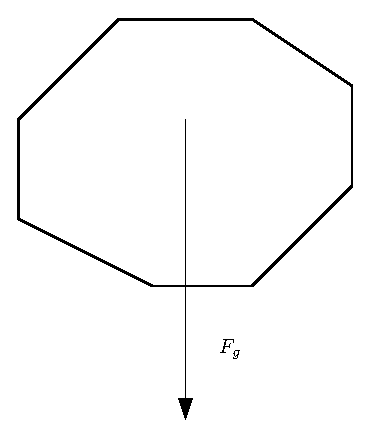
\includegraphics[]{Img/01/caida_libre}
 \caption[Ejemplo de caída libre]{ 
 Una piedra en caída libre, la única fuerza que actúa sobre ella es la de la gravedad.
 } \label{piedra:fig}
\end{figure}

En la antiguedad, Aristóteles pensaba que este movimiento era directamente proporcional a la masa.
Él afirmaba que dada una misma altura, un cuerpo con el doble de masa caería el doble de rápido.
Esta idea fue aceptada durante varios siglos.
No fue hasta la llegada del método científico que se empezó a cambiar este punto de vista.

Se cuenta una anécdota con ciertos toques de leyenda.
Se dice que Galileo dejo caer en un mismo instante una pelota de madera de un kilo de peso y una bala de cañón de diez kilos de peso desde la torre inclinada de Pisa, y la gente pudo apreciar como estos cayeron casi al mismo tiempo.
Con el simple hecho de un experimento la teoría aristotélica quedaba refutada.
Al parecer antes de los pensadores y filósofos del renacimiento, nadie se había preguntado si los conocimientos que prevalecían eran verdaderos; es decir, nadie había hecho un experimento para probar si algo era de verdad como se decía.
La simple autoridad de Aristóteles bastaba para que se diese por hecho.

Fue después de Galileo en 1685 que Newton explicó con más detalle este movimiento, con su \emph{ley de la gravitación universal}.
Newton fundamentó la mecánica con sus leyes del movimiento y la ley de la gravitación universal.
En las primeras, se dice que un objeto permanece en su estado de reposo o de movimiento rectilíneo uniforme a menos que una fuerza lo perturbe.
Esta fuerza perturbadora le produce al objeto un cambio de velocidad, es decir, una aceleración, en mecánica de Newton las fuerzas producen \emph{aceleración}.
La ley de la gravitación universal dice que todos los cuerpos se atraen.
También dice que la fuerza de atracción entre dos cuerpos es directamente proporcional al producto de sus masas e inversamente proporcional al cuadrado de sus distancias.

A partir de esta idea, si la fuerza cambia con el tiempo, también lo hará la aceleración.
Sin embargo por suerte para nosotros, el movimiento de caída libre imprime siempre \emph{aproximadamente} la misma aceleración, es decir, la fuerza de gravedad actua sobre todas las cosas con \emph{casi} la misma fuerza.
Una consecuencia de la ley de la gravitación universal y de que la masa de la Tierra sea muy grande en comparación de las cosas que estamos acostumbrados ver caer.

Gracias a que la fuerza que atrae las cosas a la tierra es casi constante, el problema de caída libre tendrá una solución matemática analítica y hasta cierto punto fácil de obtener.
Hay muchas maneras de derivar estas leyes, más adelante cuando se unan todos los modelos se entenderá por qué elegí explicarla de esta manera y no de una manera más natural.

Empiezo planteando las condiciones del modelo: suponemos que se trata de un objeto con masa $m$, que se encuentra al iniciar su movimiento a una altura $y_0$, que en el momento de iniciar su movimiento tiene una velocidad inicial $v_0$ y que durante todo su movimiento sólo va a actuar sobre él una fuerza constante $F$ (Figura~\ref{cida:fig}), que le imprime una aceleración constante $a$ y que esta fuerza es precisamente la fuerza de gravedad que ejerce la tierra sobre él, es decir: $a = g$.

\begin{figure}
 \centering
 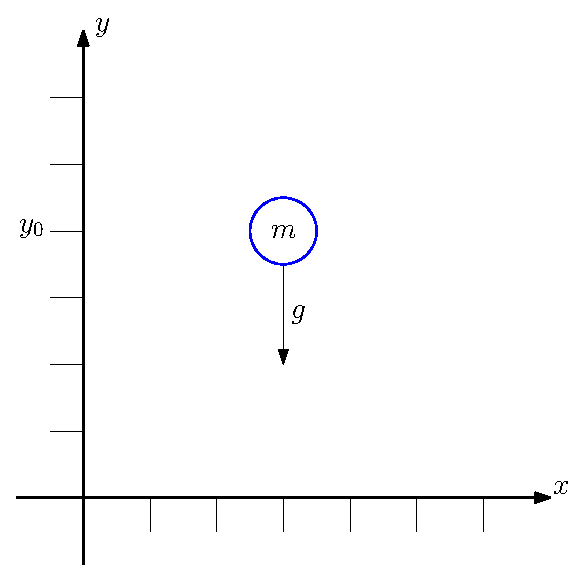
\includegraphics[]{Img/01/cuerpo_caida}
 \caption[Diagrama de cuerpo libre]{ 
 El modelo del cuerpo en caida libre, con su sistema de coordenadas.
 } \label{cida:fig}
\end{figure}

Además por seguir la convención usual, se moverá en un sistema coordenado derecho, es decir las direcciones positivas serán derecha en el eje $x$, y arriba en el eje $y$, por ende los movimientos hacia abajo y a la izquierda serán negativos, respecto a cada uno de los ejes.
Además sabemos que la gravedad sólo afecta el movimiento vertical del cuerpo, es decir sólo actúa sobre el eje $y$.
Entonces la segunda ley de Newton nos dice que:

\begin{equation} 
F = m a
\end{equation} 

Pero nosotros sabemos que la aceleración $a$, es la derivada de la velocidad $v$, respecto al tiempo $t$.
Y que la velocidad es a su vez la derivada de la posición $y$ respecto al tiempo $t$, por lo que podemos escribir la ley de Newton como:

\begin{equation}
\label{ley:Newton}
 \frac{d^2y}{dt^2} = \frac{1}{m}F(t)
\end{equation}

Además se sabe que tenemos dos condiciones iniciales, para nuestro problema:

$$ y(0) = y_0 $$
$$ v(0) = v_0 $$

Tenemos entonces una ecuación diferencial ordinaria, de segundo orden, con dos condiciones iniciales, por lo tanto podemos encontrar una solución única.

Esta ecuación es en particular, fácil de resolver debido a que la fuerza $F$ es constante.

Primero sabemos que $F(t) = -mg$, el signo es porque la gravedad actúa hacia abajo.
Y sustituyendo en la ecuación:

\begin{equation}
\label{fuerzaGravedad}
\frac{d^2y}{dt^2} = \left(\frac{1}{m}\right)\left( -mg \right) 
\end{equation}

Aquí vemos por qué Galileo encontró que la caída libre \emph{no} depende de la masa del objeto.

Si integramos la ecuación respecto a $t$.

$$ \frac{dy}{dt} = -gt + c_2 $$

Donde $c_2$ es una constante de integración, que puede encontrarse de la primera condición inicial.

$$ \frac{dy}{dt} = -gt + v_0 $$

Podemos volver a integrar la ecuación respecto a $t$ y volver a obtener la nueva constante $c_1$ de las condiciones iniciales.

\begin{eqnarray}
 y(t) & = & -\frac{gt^2}{2} + v_0t + c_1 \nonumber \\
      & = & -\frac{gt^2}{2} + v_0t + y_0
\end{eqnarray}

Que es la función que estábamos buscando, esta función nos dice cual es el valor de la coordenada $y$ del objeto cuando ha transcurrido un tiempo $t$.
Esto es precisamente lo que necesitamos saber para hacer una animación: una función que nos diga cómo se mueve algo conforme pasa el tiempo.
También cabe señalar que en nuestro caso de la caída libre $v_0 = 0$, recordemos que el cuerpo se dejó caer, por lo que nuestra función se simplifica.
Y se puede simplificar aun más, si escogemos un sistema de referencia tal que el movimiento del objeto empiece en el origen de dicho sistema es decir $y_0 = 0$.
La forma más simple de nuestra función es entonces:

\begin{equation}
 y(t) = -\frac{gt^2}{2}
\end{equation}

Quizás este sistema puede parecer un poco simple, y en efecto lo es, en el sentido que pudo resolverse sin mayor problema y de una manera analítica, esto se debió a que la aceleración, y por ende la fuerza se supuso constante.
El valor de este modelo radica más bien en la existencia de una solución analítica.

\section{El sistema masa-resorte}

Para explicar esta situación se partirá desde lo más simple a lo más complejo.
El modelo más sencillo se conoce como un \emph{oscilador armónico simple}.
Después se tratará de agregar una segunda fuerza que servirá como un amortiguador, este nuevo modelo se conoce como \emph{oscilador armónico amortiguado}.
Por último este modelo se generalizará a un sistema en tres dimensiones y con vectores y finalmente derivaremos la fórmula que ocuparemos durante el resto del trabajo. 

La mecánica de vibraciones se debe al físico inglés Robert Hooke, la vida de este científico es muy interesante por diversos motivos.\footnote{Una biografía de Hooke se puede encontrar en la \href{https://es.wikipedia.org/wiki/Robert_Hooke}{wikipedia} en español; una biografía aun más completa, en \href{https://mathshistory.st-andrews.ac.uk/Biographies/Hooke/}{MacTutor}}
Es uno de los científicos experimentales más importantes de la historia,  y sus estudios abarcan campos muy diversos como la biología, la medicina, la cronometría, la física planetaria, la microscopía, la náutica y la arquitectura. 
Estuvo en disputas con Newton por el descubrimiento de la ley de la gravitación universal.

Aquí estamos interesados en uno de sus descubrimientos en elasticidad y que es conocido como \emph{Ley de Hooke}.
Que nos dice: 
\begin{quote}
La fuerza restauradora ejercida por un resorte es linealmente proporcional al desplazamiento del resorte desde su posición de reposo y está dirigida hacia esa misma posición\footnote{En el libro~\cite{Blanchard:Ecuaciones} en el apartado dedicado a Modelación por medio de Sistemas, se enuncia de esta manera, ignoro si Hooke pensó en resortes al enunciar su ley, o se le descubrió esta aplicación en un momento posterior.}.
\end{quote}

\subsection{Oscilador armónico simple}
Imagínese que se tiene una masa sujeta por un resorte sobre la que no actúa ninguna fuerza adicional.
Por el momento vamos a suponer que no hay fricción del medio, presumiblemente el aire y que no está sujeta a la fuerza de gravedad.
Por estas condiciones ideales la masa no tendrá pérdida de energía, es decir se moverá por siempre.

De nuevo la misma idea que antes; ocuparemos la ecuación de Newton y lo único que cambiará en nuestro modelo será la expresión para calcular la fuerza, en vez de la fuerza de gravedad, se modelará la fuerza del resorte.

Imaginemos el resorte; los resortes se estiran y se comprimen cuando se les aplica una fuerza.
Siempre que pasa esto, el resorte en respuesta ejerce una fuerza restauradora, esta fuerza siempre lucha por devolver al resorte a su punto original de reposo es decir a donde no está ni comprimido ni estirado.
Es entonces que la ley de Hooke para los resortes nos da una manera de calcular esta fuerza restauradora $F_s$.

Empecemos a plantear las condiciones del modelo, supongamos que es una masa unida por un resorte a un objeto inamovible, una pared por ejemplo y que todo el sistema descansa en el piso, para que no lo afecte la gravedad, y este piso no le da ningún tipo de fricción.
En estas condiciones el único movimiento permitido para la masa será el horizontal y a la derecha, de nuevo por convención diremos que es a la dirección positiva del eje $x$.
La Figura~\ref{masaResorte:fig} ilustra la situación aquí descrita.

\begin{figure}[htb]
 \centering
 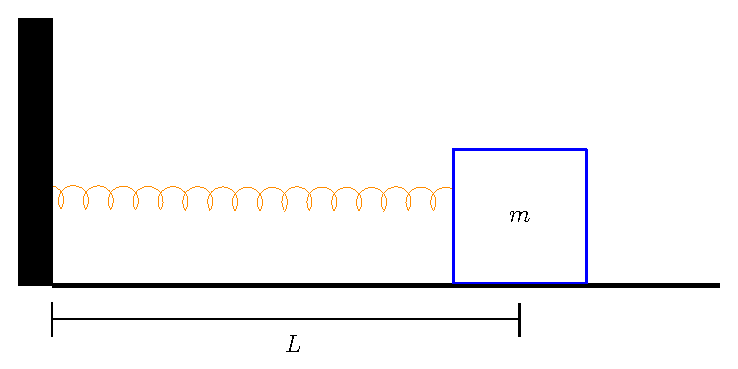
\includegraphics[width=0.6\textwidth]{Img/01/masaResorte}
 \caption[Masa unida por un resorte]{ 
 Una masa que se mueve solamente afectada por la fuerza de un resorte.
 } \label{masaResorte:fig}
\end{figure}

Se trata de modelar el movimiento de la masa a lo largo del tiempo $t$.
La masa del cuerpo de nuevo la denotaremos como $m$ y el origen del sistema será el punto donde el resorte se une a la pared.
Supongamos también que cuando el resorte está en reposo tiene un largo $L$.
La expresión que nos dice cual es la fuerza del resorte, que denotaremos como ya se dijo $F_s$, para un estiramiento razonablemente pequeño es la \emph{ley de Hooke para los resortes} y se escribe como sigue:

\begin{equation}
F_s = -k_s \left( x - L \right)
\end{equation}

Esta expresión básicamente nos dice que la fuerza es proporcional a la distancia de la masa a su punto de equilibrio donde el resorte esta en reposo.
La nomenclatura $F_s$ se debe a que la mayoría de la bibliografía consultada está en inglés y traté de ser consistente con ella, ésta es la fuerza del resorte o \emph{\foreignlanguage{english}{spring force}}.

Se observa en esta expresión que cuando el resorte está estirado, es decir, su largo $x$ es mayor a $L$ la fuerza del resorte se vuelve negativa y por ende jala a la masa a su punto de reposo.
Como se ve en la Figura~\ref{fig:estirada}.

\begin{figure}
 \centering
  \begin{subfigure}[b]{0.5\textwidth}
    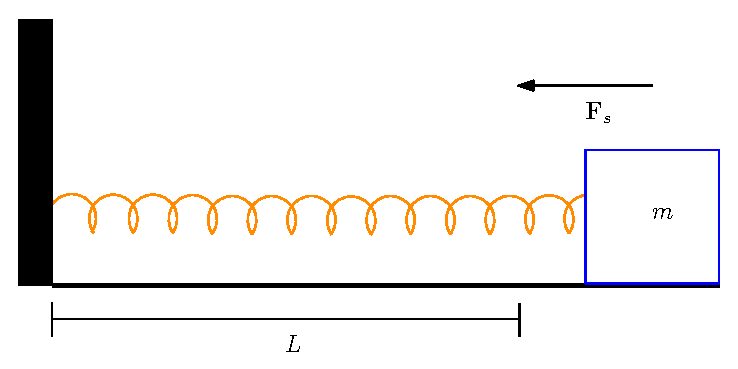
\includegraphics[width=\textwidth]{Img/01/masaEstirada}
    \caption{Cuando $x>L$, el resorte jala la masa.}
  \label{fig:estirada}
  \end{subfigure}
\\
  \begin{subfigure}[b]{0.5\textwidth}
    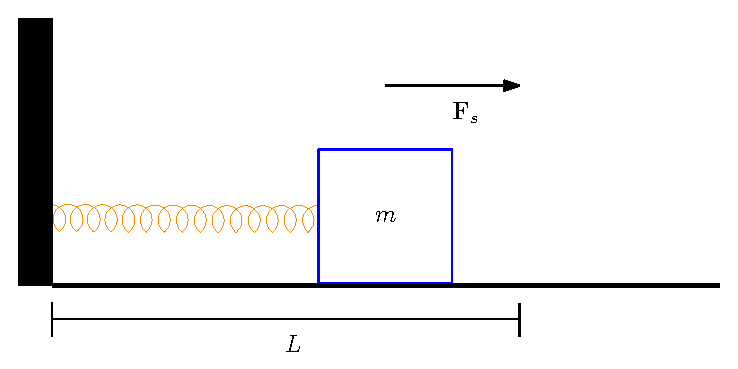
\includegraphics[width=\textwidth]{Img/01/masaCompresa}
    \caption{Cuando $x<L$, el resorte empuja la masa}
    \label{fig:compresa}
  \end{subfigure}
 \caption[Ley de Hooke para resortes]{ 
 $F_s$ trata de llevar el sistema a $x = L$
 } \label{leyHokke:fig}
\end{figure}

En el caso que el resorte esté compreso (Figura~\ref{fig:compresa}), es decir, $ x < L$, el resorte empuja el cuerpo para que alcance la posición de reposo y de nuevo lo hace con una fuerza proporcional a la distancia que esté alejado del cuerpo de este punto. 

También se observa que cuando el largo del resorte es $ x = L$ el resorte está en reposo y por lo tanto la fuerza se hace cero, éste es el caso que se ilustró en la Figura~\ref{masaResorte:fig}.

Esta expresión para la fuerza se vuelve a aplicar a la ecuación de la ley de Newton, quedando la siguiente ecuación diferencial.

\begin{eqnarray}
m \frac{d^2x}{dt^2} & = & F(t) \nonumber \\
                    & = & F_s \nonumber \\
                    & = & -k_s \left( x - L \right) \nonumber \\
\frac{d^2x}{dt^2} + \frac{k_s}{m}x  & = & \frac{k_s L}{m}
\end{eqnarray}

Esta ecuación de nuevo tendrá solución única si se especifican un par de condiciones iniciales de la forma $x(0) = x_0$ y $ v(0) = v_0 $.
La teoría de ecuaciones diferenciales nos dice que esta solución se puede encontrar, mediante la suma de una solución particular $x_p$ y una solución general de la ecuación diferencial homogénea asociada al problema $x_h$.
Es decir $x(t) = x_p + x_h$.

Por simple inspección se puede ver que $x(t)= L$ es una solución que nos puede servir como $x_p$ y afortunadamente la ecuación homogénea  es una \emph{ecuación diferencial lineal ordinaria de coeficientes constantes} por lo que es relativamente simple de resolver.
Además recuérdese que las constantes $k_s$, $m$ y $L$, son todas positivas por lo que una solución es:

\begin{equation}
x_h = c_1 \cos{\sqrt{\frac{k_s}{m}}}t + c_2 \sin{\sqrt{\frac{k_s}{m}}}t
\end{equation}

Con estas dos soluciones tenemos:
\begin{eqnarray}
x(t) & = & x_p + x_h \nonumber \\
     & = & c_1 \cos{\left(\sqrt{\frac{k_s}{m}} t \right)} + c_2 \sin{\left(\sqrt{\frac{k_s}{m}} t \right)} + L
\end{eqnarray}

Y podemos determinar las dos constantes de integración $c_1$ y $c_2$ de las condiciones iniciales.

Para este problema en particular la solución que estamos buscando es:

\begin{equation}
x(t) = \left(x_0 - L \right) \cos{\left(\sqrt{\frac{k_s}{m}} t \right)} +  \left( v_0 \sqrt{\frac{m}{k_s}}\right) \sin{\left(\sqrt{\frac{k_s}{m}} t \right)} + L
\end{equation}

Como puede apreciarse en la solución el cuerpo nunca deja de moverse, su movimiento está expresado por una función periódica.
Esto es debido a que en un medio ideal como éste el sistema no disipa energía por lo tanto, nunca cesa su movimiento, y el resorte se comprime y se estira de la misma manera por siempre.

\subsection{Oscilador armónico amortiguado}

Como es lógico las condiciones ideales antes tratadas son casi imposibles de alcanzar en la realidad, por lo que es necesario agregar a nuestro sistema una manera de perder energía.

Una manera simple de hacerlo es agregándole una resistencia por parte del medio, por ejemplo el aire, o el agua si todo el sistema se haya sumergido bajo ésta. 

Esta nueva fuerza en el sistema, a menudo se supone directamente proporcional a la velocidad del cuerpo con respecto al medio en el que se encuentra y se modela con la siguiente ecuación.

\begin{equation}
F_d = -k_d\frac{dx}{dt}
\end{equation}

El signo es negativo debido que la resistencia del medio se opone a la velocidad. Es decir trata de detener la masa poco a poco.
De nuevo una aclaración sobre la nomenclatura: se dice que está es la fuerza de amortiguación y se refiere a la palabra amortiguador en inglés: \foreignlanguage{english}{\emph{damping}}.
Y entonces el nuevo modelo toma la forma:

\begin{eqnarray}
m \frac{d^2x}{dt^2} & = & F_s + F_d \nonumber \\
& = & -k_s \left( x - L \right) -k_d\frac{dx}{dt} \nonumber \\
m \frac{d^2x}{dt^2} + k_d\frac{dx}{dt} + k_s x & = & k_s L 
\end{eqnarray}
Una vez más sujeto a las mismas condiciones iniciales $x(0) = x_0$ y $ v(0) = v_0$.

Esta ecuación se resuelve de una manera similar a la de la sección pasada, donde una solución particular $x_p$ vuelve a ser $x_p = L$.
Para encontrar una solución general se requiere resolver la ecuación homogénea asociada:

\begin{equation}
m \frac{d^2x}{dt^2} + k_d\frac{dx}{dt} + k_s x = 0
\end{equation}

De nuevo la teoría nos dice que esta ecuación tiene una solución de la forma:

\begin{equation}
x(t) = c_1 e^{n_1 x} + c_2 e^{n_2 x} \nonumber
\end{equation}

Donde las constantes $n_1$ y $n_2$ son soluciones de la ecuacion algebraica en $n$:

\begin{equation}
m n^2 +  k_d n + k_s = 0
\end{equation}

Dado que ésta es una ecuación de segundo grado, puede resolverse con la fórmula general.
Además se puede obtener información de la solución analizando cómo es $k_d^2$ con respecto a $4 m k_s$ (lo que vendría a ser $b^2$ con respecto a $4ac$).
Esto nos lleva a tres casos: que $n$ tenga dos valores reales diferentes, que $n$ tenga un solo valor real y que $n$ tenga un par de valores complejos conjugados.

Estos casos son analizados a detalle en~\cite{Ross:Ecuaciones} y por lo tanto lo único que diré es que los dos primeros casos nos llevan a resultados donde el amortiguador es tan fuerte que no deja a la masa oscilar ni siquiera una vez.
Es decir en donde la fuerza del medio es muy superior a la fuerza del resorte.

El único caso que a nosotros nos interesa es precisamente aquel donde el amortiguador es débil, y deja oscilar a la masa unas cuantas veces antes de detenerla, este caso se da precisamente cuando se trata de dos valores complejos conjugados de $n$. 

Este caso es cuando $k_d^2 < 4 m k_s$ es decir que el discriminante de la ecuación es negativo, por lo que la solución es de la forma:
\begin{eqnarray}
n_1 & = & \alpha + \beta i \nonumber \\
n_2 & = & \alpha - \beta i \nonumber
\end{eqnarray}
En donde:
\begin{eqnarray}
\alpha & = & \frac{k_d}{2m} \nonumber \\
\beta  & = & \frac{\sqrt{4 m k_s - k_d^2}}{2m} \nonumber
\end{eqnarray}
Y por tanto la ecuación diferencial tiene una solución de la forma:

\begin{equation}
\label{solOsiArmAmor} 
x(t) = e^{-\alpha t} \left( c_1 \cos{\beta t} + c_2 \sin{\beta t} \right) + L
\end{equation}

De nuevo por medio de las condiciones iniciales se pueden obtener los valores de las constantes $c_1$ y $c_2$, quedando de esta manera:

\begin{eqnarray}
c_1 & = & x_0 - L \nonumber \\
c_2 & = & \frac{v_0 + \left( x_0 - L \right) \alpha }{\beta } \nonumber 
\end{eqnarray}

De la solución \eqref{solOsiArmAmor} es claro que cuando el tiempo $t \rightarrow \infty $, el factor $e^{-\alpha t}$ dominará y la masa se detendrá poco a poco.

A manera de ejemplo ilustrativo, podemos elegir un conjunto arbitrario de valores para los parámetros. 
Por ejemplo, si $m = \frac{1}{2}$, $k_d = \frac{1}{10}$, $k_s = \frac{9 + 1 / 100}{2}$, $x_0 = 6$ y $v_0 = 9 - 3/10$.
Entonces $\alpha = \frac{1}{10}$, $\beta = 3$, $c_1 = 3$ y $c_2 = 3$.
Lo que conduce a la solución $x(t) = e^{\frac{-1}{10}t} \left( 3 \cos{t} + 3 \sin{t} \right) + 3$, cuyo comportamiento se puede ver en la Figura~\ref{OsciAmor:fig}.

\begin{figure}[htb]
 \centering
 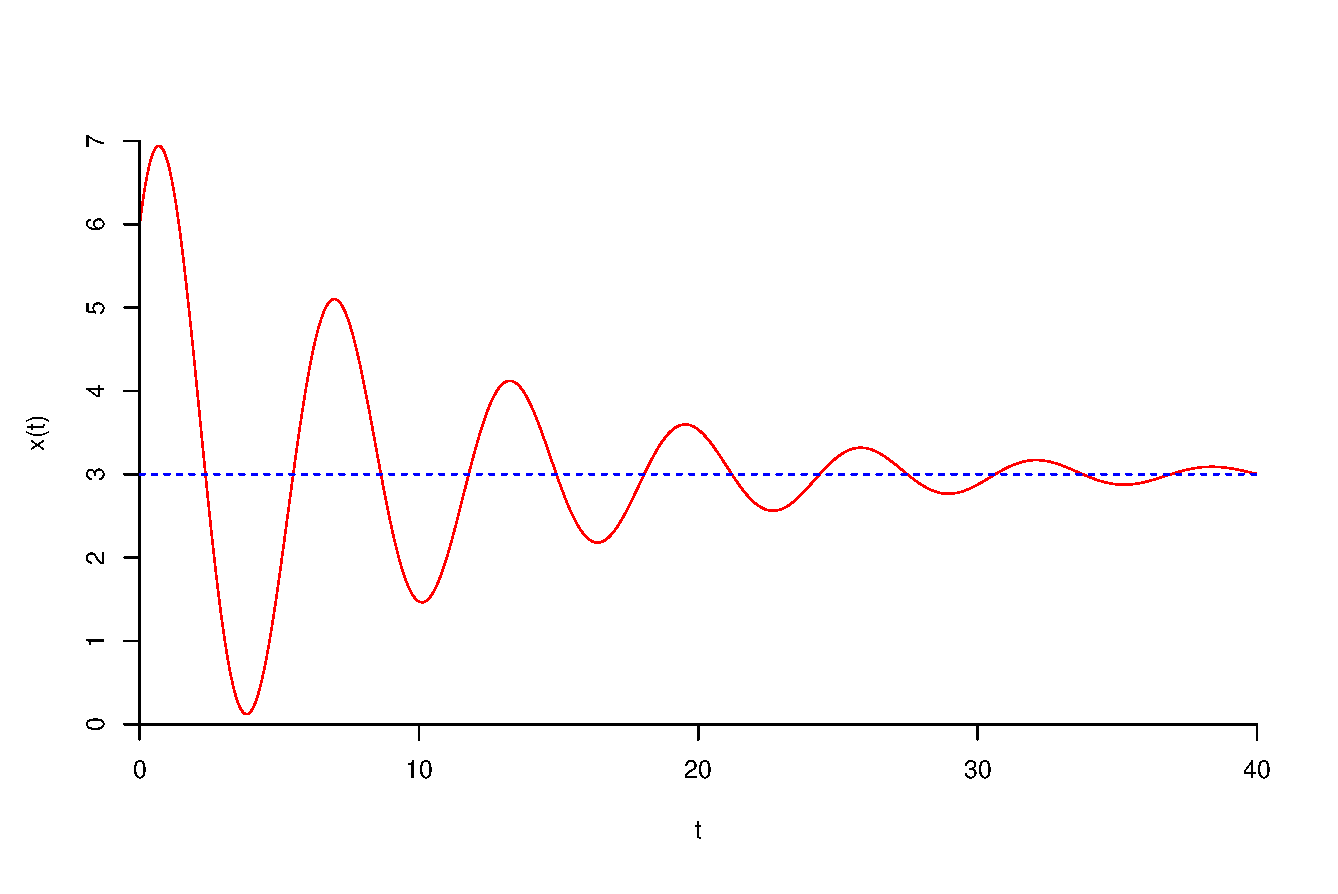
\includegraphics[width=0.85\textwidth]{Img/01/oscilador_amortiguado}
 \caption[Plano fase del oscilador armónico amortiguado]{ 
 Gráfica de $x(t) = e^{\frac{-1}{10}t} \left( 3 \cos{t} + 3 \sin{t} \right) + 3$. La linea discontinua en azul indica el estado de equilibrio: $x(t) = L$.
 } \label{OsciAmor:fig}
\end{figure}

\subsection{Masa-resorte en más de una dimensión}

Tomaremos el modelo de la sección anterior; pero lo vamos a generalizar de manera que se pueda modelar este mismo fenómeno unidimensional solo que situado en un espacio tridimensional.
Por medios geométricos trataré de aplicar las mismas fórmulas de la sección pasada.
Por simplicidad en los diagramas, voy a explicar el caso de dos dimensiones, sin embargo, como la explicación se hará con vectores, no se debe de tener problema en generalizar para tres dimensiones.

De aquí en adelante, para la notacion matemática; usaré la convención de escribir los vectores en negritas y los escalares en fuente normal~\footnote{Ésta es una convención muy aceptada en la literatura de las gráficas por computadora}.

Primero vamos a considerar que hay dos puntos en el espacio que están unidos por un resorte, este resorte es la única fuerza que actúa sobre ellos.
El resorte no tiene masa y ambos cuerpos tienen una masa $m$.
Los puntos no están sujetos, es decir se mueven libremente por el espacio, y la única fuerza que actúa sobre ellos es el resorte.

Hay que notar que a diferencia de la sección pasada, donde el resorte estaba empotrado en la pared, aquí el resorte esta unido a dos puntos sueltos, y por lo tanto aplica la misma fuerza sobre cada uno de los puntos.
Esto se puede apreciar mejor en la Figura \ref{masaSuelta:fig}.

\begin{figure}[hbt]
\centering
  \begin{subfigure}[b]{0.45\textwidth}
    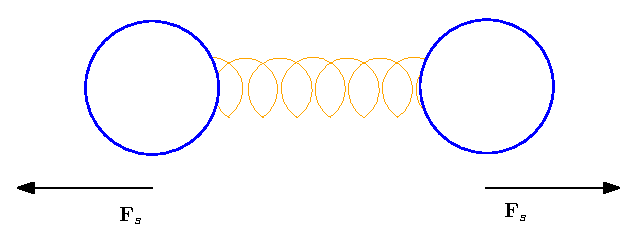
\includegraphics[width=\textwidth]{Img/01/resortesJuntos}
    \caption{Cuando $\textbf{r}<L$, el resorte empuja ambas masas}
    \label{fig:juntos}
  \end{subfigure}
\\
  \begin{subfigure}[b]{0.5\textwidth}
    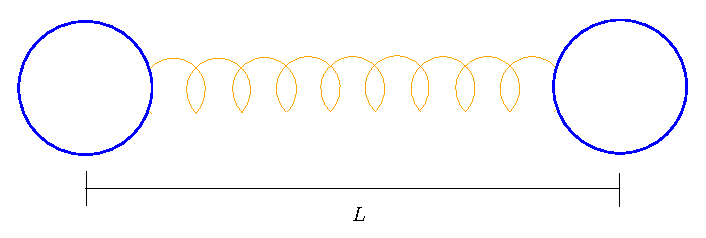
\includegraphics[width=\textwidth]{Img/01/resortesNormal}
    \caption{Cuando $\textbf{r}=L$, el resorte no ejerce fuerza}
    \label{fig:normales}
  \end{subfigure}
\\
  \begin{subfigure}[b]{0.7\textwidth}
    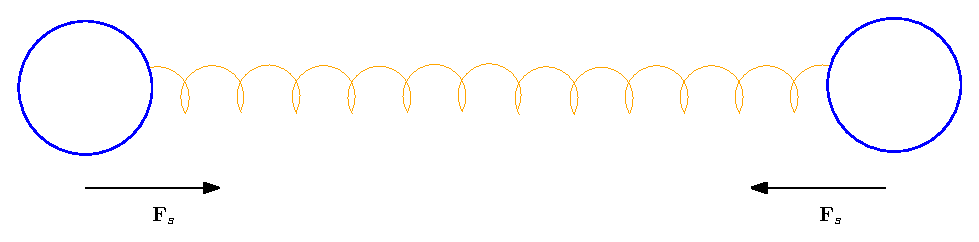
\includegraphics[width=\textwidth]{Img/01/resortesSeparados}
    \caption{Cuando $\textbf{r}>L$, el resorte jala ambas masas.}
    \label{fig:estirados}
  \end{subfigure}
 \caption[Masas libres en el espacio unidas por un resorte]{ 
 Como las masas están libres, el resorte aplica sobre cada una de ellas la misma fuerza, pero en sentido contrario.
 } \label{masaSuelta:fig}
\end{figure}

Llamaré estos puntos $a$ y $b$ respectivamente, y vemos que una posible manera de localizarlos en el espacio es el vector de posición de cada uno de ellos, denotados por $\textbf{p}_a$ y $\textbf{p}_b$.

\begin{figure}
 \centering
 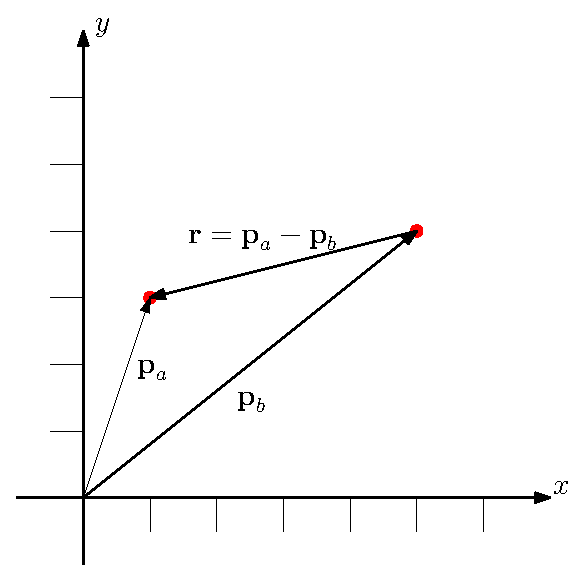
\includegraphics[width=7cm]{Img/01/vector_posicion}
 \caption[Ejemplo de vectores de posición]{ 
 Podemos localizar puntos en el espacio por medio de sus vectores de posición.
 } \label{posVec:fig}
\end{figure}

\subsubsection{La fuerza del resorte}

Vamos a calcular la fuerza del resorte sobre el punto $a$; la denotaré como $\textbf{F}_a$, y por lo anterior ya se sabe que la fuerza que actúa sobre $b$ es su negativo, es decir $\textbf{F}_b = -\textbf{F}_a$

Sabemos que una manera de encontrar el vector que une los puntos $a$ y $b$ es restando los vectores de posición de cada uno de ellos; a este nuevo vector lo llamaremos $\textbf{r}$ así que:

\begin{equation}
\textbf{r} = \textbf{p}_a - \textbf{p}_b
\end{equation}

Como se ve en la Figura~\ref{posVec:fig} este vector empieza en la punta de $\textbf{p}_b$ y termina en la punta de $\textbf{p}_a$.
Entonces la distancia que hay de $a$ a $b$ es precisamente la norma de este vector $\textbf{r}$, dicho de otra manera $\textbf{r} = \textbf{p}_a - \textbf{p}_b$ y $\overline{ab} = |\textbf{r}|$.

Ahora que sabemos la distancia de $a$ a $b$, la podemos restar con el tamaño de resorte que es el escalar $L$.
Si a este resultado lo multiplicamos por la constante del resorte $k_s$ sabremos la magnitud de la fuerza del resorte, es decir calculando $k_s \left( |\textbf{r}| - L \right)$.

Éste es un escalar, que representa la magnitud de la fuerza, pero como ésta última es un vector, hace falta que le demos dirección, para hacerlo multiplico el escalar por el vector $\textbf{r}$ normalizado.

Analizaremos la acción de la fuerza.
Si el factor $k_s \left( |\textbf{r}| - L \right)$ es negativo, entonces $| \textbf{r} | < L$, significa que el resorte está comprimido, luego entonces la fuerza debe empujar el punto $a$ lejos del punto $b$, como ya dijimos que $\textbf{r}$ representa un vector que va de $b$ a $a$, entonces la fuerza debe tener la direccion de este vector.
Veamos el caso contrario, si $ | \textbf{r} | > L $ el resorte está estirado, $k_s \left( |\textbf{r}| - L \right)$ es positivo y la fuerza debe jalar el punto $a$ en dirección de $b$, es decir en la dirección contraria que el vector $\textbf{r}$.
De estas dos observaciones nos damos cuenta de que el signo de $k_s \left( |\textbf{r}| - L \right)$ debe ser negativo, es decir:

\begin{equation}
\label{fuerza:resorte}
\textbf{F}_a = -k_s \left( |\textbf{r}| - L \right) \frac{\textbf{r}}{|\textbf{r}|}
\end{equation}

Como se dijo, sólo se ha calculado la fuerza que actúa sobre el punto $a$, sin embargo por la simetría del sistema y que ambos puntos están sueltos en el espacio, la fuerza sobre el punto $b$, es equivalente pero en sentido contrario, es decir:
$$ \textbf{F}_b = - \textbf{F}_a $$

\subsubsection{La fuerza del amortiguador}

En la sección pasada sólo modelamos la fuerza de un resorte que en esencia presenta la misma carencia del primer resorte que analizamos: le falta una manera de perder energía.
Ya habíamos analizado una manera eficaz de hacer que el oscilador disipe energía, sin embargo esto se debía al medio.
Aquí la idea es un poco diferente, vamos a pensar que esta resistencia no está presente en el medio, sino en el mismo resorte en sí; es decir nuestro resorte además de ser tal será un amortiguador, y la resistencia actuará por lo tanto en la misma línea de acción del resorte.

Ya dijimos anteriormente que esta resistencia la vamos a suponer proporcional a la velocidad.
Y con la misma idea que antes vamos a agregarla al modelo anterior.
Ya sabemos que tenemos una manera de localizar a los puntos $a$ y $b$ en el espacio, su vector de posición, sin embargo aún no tenemos una manera de saber la velocidad de los puntos en el espacio, por ello vamos a crear dos vectores $\textbf{v}_a$ y $\textbf{v}_b$, que contienen la velocidad a la que se mueven estos puntos respectivamente.

Procedamos a calcular la fuerza que actúa sobre el punto $a$.
Esta fuerzas son: la fuerza anterior debida al resorte que los une, y una nueva fuerza ahora debida al amortiguador.

\begin{equation}
\textbf{F}_a = \textbf{F}_s + \textbf{F}_d
\end{equation}

Donde $\textbf{F}_s$ es precisamente la expresión \eqref{fuerza:resorte}. Así que sólo nos falta calcular $\textbf{F}_d$.
Esta fuerza, como ya se dijo, es proporcional a la velocidad a la que se mueve un punto respecto al otro $\left( \textbf{v}_a - \textbf{v}_b \right)$ con una constante $k_d$, y además actúa en el sentido contrario al de la velocidad, es decir $F_d$ es proporcional a $-k_d \left( \textbf{v}_a - \textbf{v}_b \right)$.


Ahora hay que notar también que la posición de un punto no necesariamente tiene que ver con su velocidad, es decir un punto en una misma posición se podría mover bien a una velocidad $\textbf{v}$ u a otra muy diferente, sin tener que cambiar su vector de posición.

Como ya dijimos que para nosotros el amortiguador está en el resorte, es necesario entonces trasladar esta fuerza a donde está el resorte, es decir a $\textbf{r} = \textbf{p}_a - \textbf{p}_b$.
Para hacer esto vamos a ocupar la conocida forma de la proyección de un vector sobre otro.

Sabemos que un vector $\textbf{A}$ se puede proyectar sobre un vector $\textbf{B}$ y se denota como $\mathrm{Proy}_{ \textbf{B} } \textbf{A}$ podemos obtener su magnitud con la siguiente fórmula:

\begin{equation}
| \mathrm{Proy}_{\textbf{B}} \textbf{A} | = \frac{ \textbf{A} \cdot \textbf{B} }{| \textbf{B} |}
\end{equation}

Ahora entonces calculemos la magnitud de la proyeccion del vector $\left( \textbf{v}_a - \textbf{v}_b \right)$ sobre el vector donde está el resorte, es decir sobre el vector $\textbf{r} = \textbf{p}_a - \textbf{p}_b$.
Quedando de esta manera:

\begin{equation}
 | \mathrm{Proy}_{ \textbf{r} } \textbf{v} | = \left[ \frac{ ( \textbf{v}_a - \textbf{v}_b ) \cdot ( \textbf{p}_a - \textbf{p}_b ) }{ | \textbf{p}_a - \textbf{p}_b | } \right]
\end{equation}

Sin embargo, esta cantidad es un escalar así que necesitamos multiplicarla por un vector unitario para darle dirección.
Como esta fuerza es debida al \emph{resorte-amortiguador} y está en su misma línea de acción, la multiplicamos por $\textbf{r}$ normalizado.
Quedando la expresión final para $\textbf{F}_d$:

\begin{equation}
\textbf{F}_d = - k_d \left[ \frac{ ( \textbf{v}_a - \textbf{v}_b ) \cdot ( \textbf{p}_a - \textbf{p}_b ) } { | \textbf{p}_a - \textbf{p}_b |} \right] \left[ \frac{ \textbf{p}_a - \textbf{p}_b } { | \textbf{p}_a - \textbf{p}_b |} \right]
\end{equation}

Como ya expliqué antes ésta es sólo la fuerza del amortiguador así que la expresión de fuerza para este \emph{resorte-amortiguador} (remplazando $\textbf{r} = \textbf{p}_a - \textbf{p}_b$ y $\textbf{v} = \textbf{v}_a - \textbf{v}_b$ para no hacer muy compleja la notación) es la siguiente:

\begin{eqnarray}
\textbf{F}_a & = & \textbf{F}_s + \textbf{F}_d \nonumber \\
\textbf{F}_a & = & -k_s \left( |\textbf{r}| - L \right) \frac{\textbf{r}}{|\textbf{r}|} - k_d \left[ \frac{ \textbf{v} \cdot \textbf{r} }{ |\textbf{r}|} \right] \left[ \frac{\textbf{r}} {|\textbf{r}|}\right] \nonumber \\
\label{fuerzaResorte}
\textbf{F}_a & = & - \left\{ k_s \left( |\textbf{r}| - L \right) + k_d \left[ \frac{ \textbf{v} \cdot \textbf{r} }{ |\textbf{r}|} \right] \right\} \left[ \frac{\textbf{r}} {|\textbf{r}|} \right] \\
\textbf{F}_b & = & -\textbf{F}_a \nonumber
\end{eqnarray}

\section{El modelo del gas ideal}

Aquí se va a tratar de agregar al modelo, una fuerza de presión.
La idea de esta fuerza es tomada del artículo de Matika \cite{Matyka:Presion}, y se basa en implementar un modelo simple de gas.
Este modelo cuenta con la ventaja de la sencillez, tanto en su implementación como en la rapidez de su ejecución, lo que lo hace un modelo ideal para una animación en tiempo real.

Vamos a empezar por imaginar un cuerpo cerrado en tres dimensiones, por ejemplo una esfera o un cubo, luego vamos a imaginar que la envolvente de ese cuerpo, es decir la superficie que lo cierra, es una superficie elástica, que se puede estirar y deformar, y por último supongamos que dentro de ese cuerpo, en vez de haber un vacío, hay un gas; ésta es la idea principal del modelo que trataremos de ahora en adelante, y es el motivo de estudio de este trabajo.

En las dos secciones anteriores hemos tratado los modelos que nos pueden servir como la envolvente de este cuerpo (podria ser una envolvente formada por una membrana de puntos unidos por resortes), pero hablaré mas de esto en el siguiente capitulo.
Así que sólo falta tratar el modelo de un gas por separado, para terminar nuestro tratamiento de modelos simples.
El modelo que vamos a estudiar es el del \emph{gas ideal}.

\subsection{La termodinámica}

Habíamos estado hablando de leyes de mecánica, sin embrago este modelo pertenece a una rama diferente de la física, la \emph{termodinámica}.
La termodinámica es la rama de la física que estudia los efectos de los cambios de temperatura, calor y presión, en un sistema, por medio de métodos estadísticos.\footnote{En esta definición de \emph{termodinámica} comúnmente se aplican modelos más complejos que el usado aquí, que sí requieren de métodos estadísticos, pero de hecho nuestro modelo es en esencia determinista.}

El estudio de la termodinámica empieza con el descubrimiento de las maneras de medir el calor, es decir, con la invención de los primeros termómetros, fue así como se notó que existen sistemas que presentan cambios cualitativos, cuando cambian su temperatura.

Uno de estos sistemas es el gas, y por lo tanto existen algunos modelos para estudiar las propiedades de los gases.
El más simple de estos modelos es el modelo del gas ideal, que se define por medio de la \emph{ley de los gases ideales}, que no es otra cosa que la ecuación de estado de un gas ideal.

\subsection{Un modelo simple}

Al principio, para poder estudiar un fenómeno del cual no se conocen muchas cosas, es común relajar muchas de sus propiedades e idealizar muchas situaciones, es decir construir modelos simples, en este caso nos abocamos al primer modelo que se construyó para un gas, y por lo mismo está sujeto a muchas suposiciones que en la realidad nunca son alcanzadas por ningún gas, de ahí que lo llamaran \emph{gas ideal}.

En física y en química, una ecuación de estado es una ecuación que describe el estado de agregación de la materia en función de ciertos parámetros, es decir determina la relación matemática entre dos o más funciones de estado asociadas con la materia.

En nuestro caso queremos describir el estado de un gas en función de propiedades macroscópicas del mismo.
Estas propiedades son: la temperatura, el volumen, la presión y el número de moléculas.

Por medio de resultados experimentales se determinó la primera ecuación de estado, una explicación de cómo se hicieron estos experimentos y se llegó a ella se puede encontrar en~\cite{Resnick:Fisica}, pero a nosotros nos bastará con conocerla:

\begin{eqnarray}
PV & = & nRT \nonumber \\
P & = & \frac{1}{V}nRT
\end{eqnarray}

En donde $P$ es la presión del gas, $V$ es el volumen del gas, $n$ es el número de moles, $R$ es una constante llamada constante del gas ideal y $T$ es la temperatura.
La constante $R$ es la multiplicación de la constante de Boltzman y el número de Avogadro~\footnote{Esta constante universal aparece en varias ecuaciones importantes de la termodinámica, es equivalente a la constante de Boltzman pero expresada en unidades de energia.}.
Las unidades de esta constante son Joule ($J$) sobre mol ($mol$) Kelvin ($K$).

$$ R = N_A k = 8.3145 \ \frac{J}{mol \cdot K}$$

Esta ecuación de estado es un aproximación bastante buena cuando se trata de gases a bajas densidades, y la experimentación nos muestra que en estas condiciones \emph{todos} los gases tienden a comportarse como este gas ideal.

\subsection{La presión de un gas}

La presión no es en sí una fuerza sino es una fuerza aplicada en una unidad de área, y por eso se mide en una unidad llamada \emph{Pascals} (Pa) y no en Newtons (N) que es la unidad en que se mide la fuerza.
Entonces, si $\textbf{P}$ es la presion, $\textbf{F}$ es una fuerza y $A$ el área donde se está aplicando esta fuerza:

$$ \textbf{P} = \frac{\textbf{F}}{A} $$

De tal manera que si nosotros queremos una \emph{fuerza de presión}, para poder acumularla en la ecuación de Newton; como lo hicimos con las fuerzas anteriores necesitamos multiplicarla por el área de aplicación.
Dicho de otra manera:

$$ \textbf{F}_p = \textbf{P} \cdot A $$

Donde $\textbf{F}_p$ es la fuerza de presión que estamos buscando, $A$ es el área de aplicación y $\textbf{P}$ es el vector que representa la presión.
Ya se dijo que la magnitud de la presión puede calcularse con la ecuación de estado, pero no se ha dicho qué dirección lleva.
La presión actúa sobre la superficie de la cara del cuerpo, y es siempre de normal a esta cara, de manera que la presión es:

$$ \textbf{P} = P \cdot \textbf{n} $$

En donde $P$ es el escalar calculado con la ecuación de estado y $\textbf{n}$ es un vector unitario normal a la cara sobre la que se está calculando la presión.

Para nuestro modelo se debe tomar en cuenta que sólo nos interesa calcular la fuerza de presión, de esta manera se procede de la siguiente manera.

$$ P = \frac{1}{V} \; nRT $$

De esta manera $\textbf{P}$ es:

$$ \textbf{P} = \frac{1}{V} \; nRT \left[ \textbf{n} \right] $$

Y este vector $\textbf{P}$ se usará a su vez, para obtener el vector fuerza, es decir:

$$ \textbf{F}_p = \frac{1}{V} \; nRT \left[ \textbf{n} \right] A $$

Reacomodando esta ecuación, se tiene:

$$ \textbf{F}_p = \left[ \frac{1}{V}A \; nRT \right] \textbf{n} $$

Donde para \emph{nuestro} modelo el escalar $nRT$ es un parámetro a determinarse experimentalmente, está formado por la temperatura que consideramos constante, el número molar del gas, que debe depender del gas y por la constante del gas ideal. 
Así que los tres son agrupados en una sola constante, que nosotros por ser consistentes con nuestra nomenclatura llamaremos $k_g$

De manera que: 

\begin{equation}
\label{fuerzaGas}
\textbf{F}_p = \left[ \frac{1}{V}A \; k_g \right] \textbf{n}
\end{equation}

Donde $\textbf{F}_p$ es la fuerza que deseamos acumular en cada partícula, $V$ es el volumen total de nuestro cuerpo cerrado, $A$ es el área de la cara sobre la que estamos calculando la presión, $\textbf{n}$ es un vector unitario normal a esta cara y $k_g$ es una constante positiva a ser determinada experimentalmente.
Es la ecuación que nos servirá en nuestro modelo.

\subsection{Un ejemplo ilustrativo}

Supongamos que se tiene una caja cerrada cuya \emph{tapa} tiene el largo y el ancho mostrado en la Figura~\ref{cuadrilatero:fig} la caja tiene una altura igual a 1, es decir, $h=1$. Esta caja tiene las tapas fijas a lo alto, por lo que la fuerza de un gas solo la puede deformar en sus lados.
Calculemos ahora la fuerza debida a la presión de un gas que esté dentro de esta caja.

\begin{figure}
 \centering
 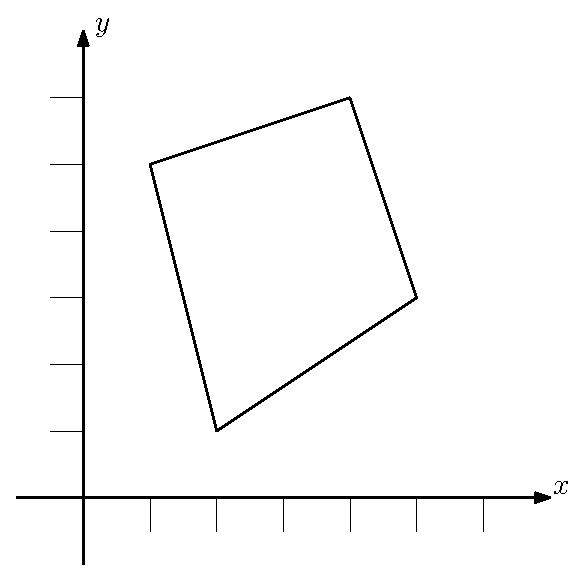
\includegraphics[width=7cm]{Img/01/cuadrilatero}
 \caption[Cuadrilátero]{ 
 La figura cerrada para la cual se harán los cálculos de presión.
 } \label{cuadrilatero:fig}
\end{figure}

Vamos a calcular la fuerza correspondiente a la presión, por medio de la ecuación \eqref{fuerzaGas}.
Como la caja es de altura unitaria, el volumen $V$ que es igual al área de su tapa por la altura equivale simplemente al área de su tapa.
Por la misma razon las áreas de las caras laterales de la caja equivalen a la longitud de el lado de la tapa en el que se encuentran.

Para calcular la fuerza de presión en este caso se necesita saber entonces: la longitud de cada uno de los lados del cuadrilátero, un vector normal a cada una de sus lados y su área.
Por suerte para nosotros lo único que necesitamos para conocer todos estos datos, es ubicar la posición de cada una de sus esquinas.

Identificaremos cada una de las esquinas $\textbf{A}_i$ por medio de sus coordenadas $x_i$ y $y_i$, dicho de otra manera $\textbf{A}_i = ( x_i , y_i)$.
Esta situación queda determinada por la Figura~\ref{cuadrilateroDiagrama:fig}.

\begin{figure}
 \centering
 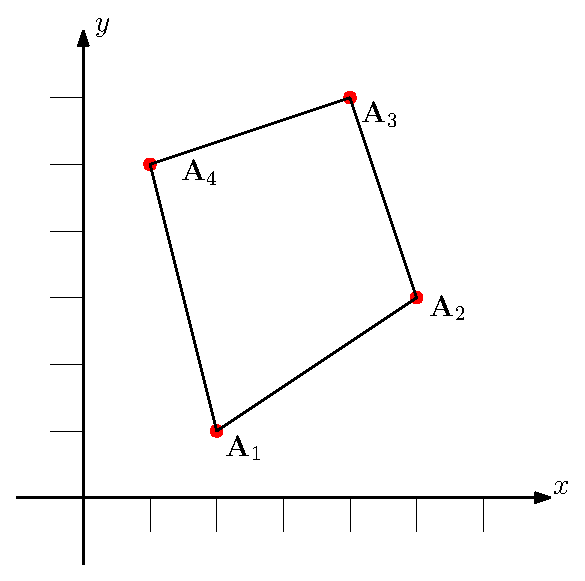
\includegraphics[width=7cm]{Img/01/cuadrilatero_diagrama}
 \caption[Cuadrilátero localizado en el espacio]{ 
 Figura con los puntos que representan las esquinas identificados y localizados.
 } \label{cuadrilateroDiagrama:fig}
\end{figure}

De donde podemos conocer, gracias al sistema de referencia, las coordenadas de cada uno de los puntos en donde se ubican las esquinas:

\begin{eqnarray}
\textbf{A}_1 & =  (x_1, y_1)  = & (2,1) \nonumber \\
\textbf{A}_2 & =  (x_2, y_2)  = & (5,3) \nonumber \\
\textbf{A}_3 & =  (x_3, y_3)  = & (4,5) \nonumber \\
\textbf{A}_4 & =  (x_4, y_4)  = & (1,4) \nonumber
\end{eqnarray}

Una vez conocidos estos datos podemos calcular la longitud de cada lado simplemente obteniendo la distancia entre dos puntos.

\begin{eqnarray}
\overline{\textbf{A}_1 \textbf{A}_2} & =  \sqrt{(x_1 - x_2)^2 + (y_1 - y_2)^2}  = & \sqrt{13}  \nonumber \\
\overline{\textbf{A}_2 \textbf{A}_3} & =  \sqrt{(x_2 - x_3)^2 + (y_2 - y_3)^2}  = & \sqrt{5}   \nonumber \\
\overline{\textbf{A}_3 \textbf{A}_4} & =  \sqrt{(x_3 - x_4)^2 + (y_3 - y_4)^2}  = & \sqrt{10}  \nonumber \\
\overline{\textbf{A}_4 \textbf{A}_1} & =  \sqrt{(x_4 - x_1)^2 + (y_4 - y_1)^2}  = & \sqrt{10}  \nonumber
\end{eqnarray}

También podemos calcular el área de la tapa con un sencillo truco, podemos trazar la diagonal que divide al cuadrilátero tal que pase por $\textbf{A}_1$ y $\textbf{A}_3$, con lo que para calcular el área total del cuadrilátero basta con calcular el área de los dos triángulos $\bigtriangleup \textbf{A}_1 \textbf{A}_3 \textbf{A}_4$ y $\bigtriangleup \textbf{A}_1 \textbf{A}_2 \textbf{A}_3$ y luego sumar ambas áreas (ver la Figura~\ref{vectorArista:fig}).

\begin{figure}
 \centering
 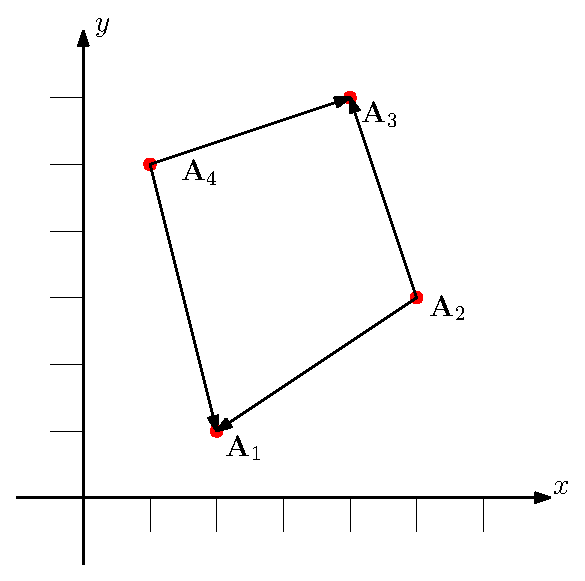
\includegraphics[width=7cm]{Img/01/vectores_cuerpo}
 \caption[Cálculo del área de un caudrilátero]{ 
Aquí se pueden ver los vectores que representan cada uno de los lados, y que son calculados por la resta de los vectores de posición de los puntos.
 } \label{vectorArista:fig}
\end{figure}

Para calcular el área del triángulo $\bigtriangleup \textbf{A}_1 \textbf{A}_3 \textbf{A}_4$ tomamos a $\textbf{A}_4$ como origen y calculamos el vector que va de $\textbf{A}_4$ a $\textbf{A}_1$, luego calculamos el vector que va de $\textbf{A}_4$ a $\textbf{A}_3$, y por último calculamos el producto cruz, tomamos su norma y lo dividimos entre dos.\footnote{Este es un teorema muy conocido de la geometría vectorial y se puede ver en cualquier libro que incluya una introducción a los vectores, me imagino que no necesito citar alguna fuente en especial}
De manera análoga para el siguiente triángulo:

El cálculo de los vectores es el siguiente:
\begin{eqnarray}
\overrightarrow{A_4 A_1} & = \textbf{A}_1 - \textbf{A}_4 = & (1, -3) \nonumber \\
\overrightarrow{A_4 A_3} & = \textbf{A}_3 - \textbf{A}_4 = & (3, 1) \nonumber \\
\overrightarrow{A_2 A_1} & = \textbf{A}_1 - \textbf{A}_2 = & (-3, -2) \nonumber \\
\overrightarrow{A_2 A_3} & = \textbf{A}_3 - \textbf{A}_2 = & (-1, 2) \nonumber
\end{eqnarray}

Y por lo explicado anteriormente el área total de la tapa $A_T$ es:

$$ A_T = A_{\bigtriangleup \textbf{A}_1 \textbf{A}_3 \textbf{A}_4} + A_{\bigtriangleup \textbf{A}_1 \textbf{A}_2 \textbf{A}_3} $$
$$ A = \frac{1}{2} | \overrightarrow{\textbf{A}_4 \textbf{A}_1} \times \overrightarrow{\textbf{A}_4 \textbf{A}_3} | + \frac{1}{2} | \overrightarrow{\textbf{A}_2 \textbf{A}_1} \times \overrightarrow{\textbf{A}_2 \textbf{A}_3} |$$
$$A = \frac{1}{2} | 10 | + \frac{1}{2} | -8 |$$
$$A = 9$$

Ahora sólo nos falta calcular la fuerza $\textbf{F}_p$ y acumularla en cada una de las caras laterales de la caja. Para esto y sólo por simplicidad supongamos que escogemos $k_d = 10$ entonces el cálculo de la fuerza debe hacerse por separado para cada una de las caras laterales (que en nuestro caso equivalen a los lados de la tapa):

\begin{eqnarray}
F_{\overline{\textbf{A}_1 \textbf{A}_2}} & =  \frac{1}{V}\overline{\textbf{A}_1 \textbf{A}_2} k_g & = \frac{1}{9} \sqrt{13} \left( 10 \right) \nonumber \\
F_{\overline{\textbf{A}_2 \textbf{A}_3}} & =  \frac{1}{V}\overline{\textbf{A}_2 \textbf{A}_3} k_g & = \frac{1}{9} \sqrt{5}  \left( 10 \right) \nonumber \\
F_{\overline{\textbf{A}_3 \textbf{A}_4}} & =  \frac{1}{V}\overline{\textbf{A}_3 \textbf{A}_4} k_g & = \frac{1}{9} \sqrt{10} \left( 10 \right) \nonumber \\
F_{\overline{\textbf{A}_4 \textbf{A}_1}} & =  \frac{1}{V}\overline{\textbf{A}_4 \textbf{A}_1} k_g & = \frac{1}{9} \sqrt{10} \left( 10 \right) \nonumber
\end{eqnarray}

Con lo que tenemos la magnitud de las fuerzas que actúan en cada cara, así que sólo falta calcular un vector unitario normal a la cara correspondiente para poder acumular su fuerza.

Afortunadamente, para calcular un vector normal en dos dimensiones, tenemos un método sencillo, el producto punto de dos vectores normales entre sí debe de dar cero, así que si queremos un vector normal al vector $\textbf{v}=(x, y)$ simplemente construimos uno tal que su producto punto con el primero siempre sea igual a cero, por ejemplo $\textbf{v}^n = (-y, x)$.
Con esto sabemos que el vector $\textbf{v}^n$ es siempre normal al vector $\textbf{v}$, de hecho en dos dimensiones sólo este vector y sus múltiplos son normales a $\textbf{v}$.

Sabiendo todo lo anterior, ya se puede acumular la fuerza correspondiente sobre cada cara. Por ejemplo, sobre la primera cara que está definida por el segmento que une a $\textbf{A}_1$ y $\textbf{A}_2$.
Como en el paso anterior ya se había calculado el vector $\overrightarrow{\textbf{A}_2 \textbf{A}_1} = (-3,-2)$ que en sí representa a la cara, podemos calcular su vector normal con la fórmula anterior.
Para esta cara el vector $\textbf{n}=(2,-3)$ es el vector normal, para hacerlo unitario lo dividimos entre su norma $\frac{\textbf{n}}{|\textbf{n}|} = \frac{1}{\sqrt{13}} (2, -3)$.
Y finalmente el vector fuerza que estamos buscando para esta cara en particular es:

$$\textbf{F}_{\overline{\textbf{A}_1 \textbf{A}_2}} = \frac{1}{V}\overline{\textbf{A}_1 \textbf{A}_2} k_g \vec{n} = \frac{1}{9} \sqrt{13} \left( 10 \right)  \frac{1}{\sqrt{13}} (2, -3) = \frac{10}{9}(2, -3) $$

Una consideración más que debe tenerse, al calcular el vector normal, pudiera darse el caso que éste dirija la fuerza al contrario de como se desea, es decir que la dirija, al centro del cuerpo en vez de hacia afuera.
Como se ilustra en la Figura \ref{presionMal:fig}.
En cuyo caso hay que multiplicar este vector normal por $-1$.
En general la mejor práctica es graficar el cuerpo para así poder calcular el vector normal correcto.

Por ejemplo, al calcular un vector normal para la segunda cara podríamos vernos tentados a repetir el cálculo, ocupando el vector que acabamos de calcular $\overrightarrow{\textbf{A}_4 \textbf{A}_1}$ pero al ocupar la fórmula, nos daría $n=(3,1)$ que en efecto es un vector normal a $\overrightarrow{\textbf{A}_4 \textbf{A}_1}$ pero que apunta hacia el centro del cuerpo, y por lo tanto sería incorrecto ocuparlo para dirigir la fuerza de presión.
El vector correcto para este caso es $-n = (-3,-1)$.
Así que se debe tener cuidado al calcular el vector para dirigir la fuerza de presión.

\begin{figure}
 \centering
 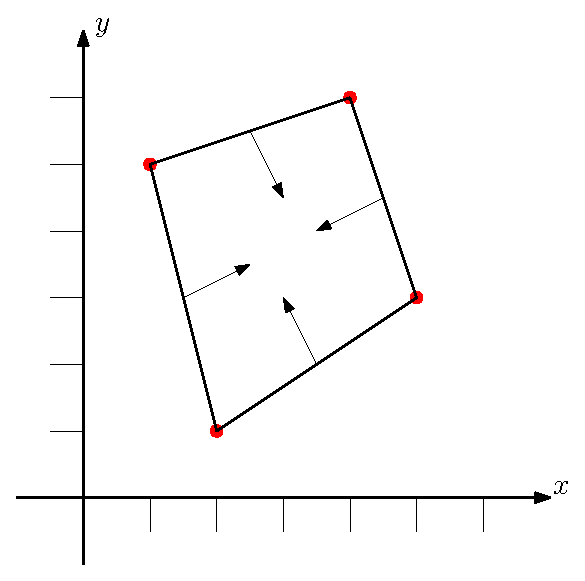
\includegraphics[width=7cm]{Img/01/presion_mal}
 \caption[Vectores de presión incorrectos]{ 
 Aqui se pueden ver los vectores incorrectos para dirigir la presión pues apuntan al centro de la figura.
 } \label{presionMal:fig}
\end{figure}

El resto de las operaciones correspondientes al ejemplo se pueden ver en el Cuadro ~\ref{ejemplo:presion}.
En la primera columna de la tabla se muestra la cara a la que se estaba calculando la fuerza, después se muestra el valor escalar de la presión, luego el vector asociado a la cara, que ya habíamos obtenido, después el vector normal resultado del procedimiento antes explicado.
Hay que tomar en cuenta que el vector podría ser que apunte hacia afuera o hacia adentro, y en la tabla ya fue corregido (multiplicándolo por el escalar $-1$).
Y en la última columna aparecen los vectores de fuerza que se estaban buscando, y son los que se requieren para poder acumularse en la ecuación de Newton.

\begin{table}
\ra{1.3}
\begin{center}
\begin{tabular} {@{}lllll@{}}
\toprule
Cara & Fuerza de Presión &  Vector de la cara & Vector Normal & Vector Fuerza \\ \midrule
$\overline{A_1A_2}$ & $\frac{1}{9} \cdot 10 \cdot \sqrt{13} $ & $\overrightarrow{A_2A_1} = (-3,-2)$ & $(\frac{2}{\sqrt{13}}, \frac{-3}{\sqrt{13}})$ & $(\frac{20}{9}, \frac{-30}{9})$ \\
$\overline{A_2A_3}$ & $\frac{1}{9} \cdot 10 \cdot \sqrt{5} $ & $\overrightarrow{A_2A_3} = (-1,2)$ & $(\frac{2}{\sqrt{5}}, \frac{1}{\sqrt{5}})$ & $(\frac{20}{9}, \frac{10}{9})$ \\
$\overline{A_3A_4}$ & $\frac{1}{9} \cdot 10 \cdot \sqrt{10} $ & $\overrightarrow{A_4A_3} = (3,1)$ & $(\frac{-1}{\sqrt{10}}, \frac{3}{\sqrt{10}})$ & $(\frac{-10}{9}, \frac{30}{9})$ \\
$\overline{A_1A_4}$ & $\frac{1}{9} \cdot 10 \cdot \sqrt{10} $ & $\overrightarrow{A_4A_1} = (1,-3)$ & $(\frac{-3}{\sqrt{10}}, \frac{-1}{\sqrt{10}})$ & $(\frac{-30}{7}, \frac{-10}{9})$ \\ 
\bottomrule
\end{tabular}
\end{center}
\caption[Ejemplo sobre cómo calcular la fuerza de presión]{Cálculo de la Fuerza de Presión, para el ejemplo}
\label{ejemplo:presion}
\end{table}

La fuerza de presión es mucho más compleja de calcular que las fuerzas debidas a la gravedad y a los \emph{resortes-amortiguadores}.
La principal dificultad es que debe tratar con la geometría del cuerpo para calcularla, además es necesario conocer el volumen total del cuerpo, y por cada cara que se acumule se debe de conocer: el área de la misma y un vector normal, por lo que a diferencia de los casos anteriores no hay una manera general de enunciar las fórmulas sino que debe analizarse el caso particular de la geometría del cuerpo que se esté tratando.


\begin{figure}
 \centering
 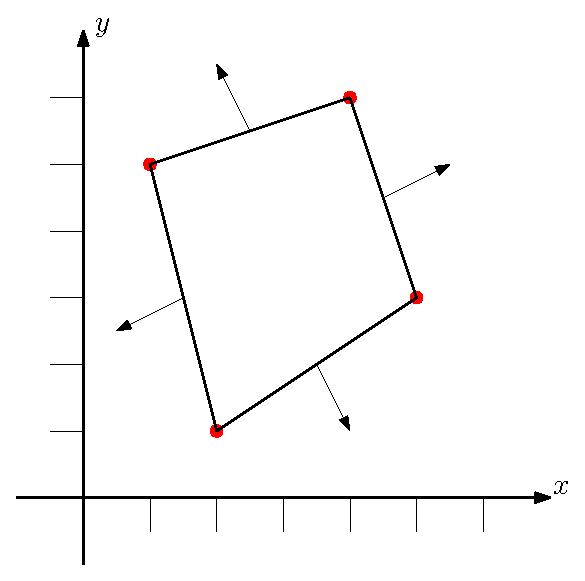
\includegraphics[width=7cm]{Img/01/presion_bien}
 \caption[Vectores de presión correctos]{ 
 Así es como debe de dirigirse la fuerza de presión. Obsérvese que cada esquina debe acomular la fuerza de las dos caras laterales que está uniendo.
 } \label{presionBien:fig}
\end{figure}
